%%%% Header %%%%%%%%%%%%%%%%%%%%%%%%%%%%%%%%%%%%%%%%%%%%%%%%%%%%%%%%%%%%%%%%%%%

\documentclass{beamer}

%%%% Packages %%%%%%%%%%%%%%%%%%%%%%%%%%%%%%%%%%%%%%%%%%%%%%%%%%%%%%%%%%%%%%%%%

% font/encoding
\usepackage[utf8]{inputenc} % .tex-file text encoding
\usepackage[T1]{fontenc} % vector fonts and hiQual special chars in output
\usepackage{libertine} % libertine font family
\usepackage[libertine]{newtxmath} % libertine mathematics
\usepackage[scaled=0.85]{inconsolata} % monospace font

% localization
\usepackage[english]{babel} % document language/localization

% maths
\usepackage{amsmath} % various maths features
\usepackage{mathtools} % aligned matrices

% figures
\usepackage{graphicx} % include external images
\usepackage[compatibility=false, labelformat=empty, justification=centering]{caption} % figure captions
\usepackage{subcaption} % captions for subfigures

% bibliography
\usepackage[style = authoryear,
            backend = biber,
            bibencoding = utf8,
            doi = false,
            isbn = false]{biblatex}

%%%% General layout %%%%%%%%%%%%%%%%%%%%%%%%%%%%%%%%%%%%%%%%%%%%%%%%%%%%%%%%%%%

% colours
\definecolor{maincol}{RGB}{46, 69, 136} % main deco colour
\usecolortheme{dove} % black/grey colours
% font
\usefonttheme{serif} % use serif fonts
\setbeamerfont{frametitle}{series=\bfseries}
% inner theme
\useinnertheme{rectangles}
% header
\useoutertheme{miniframes} % nice shading in header
\setbeamertemplate{headline}{} % disable section tree
\setbeamercolor{frametitle}{fg=white, bg=maincol}
% footline
\setbeamertemplate{navigation symbols}{} % no nav symbols
\setbeamertemplate{footline}[page number] % page number
% figures
\setkeys{Gin}{width=1.0\textwidth} % figures fill textwidth
\setbeamertemplate{caption}{\insertcaption} % no caption label
\setbeamertemplate{caption label separator}{}
% list
\setbeamertemplate{itemize items}[triangle] % list symbol
% bibliography
\setbeamertemplate{bibliography item}{} % no bibliography icon
% pdf
\hypersetup{pdfstartview={Fit}} % fit the presentation to the window
% box colours
\setbeamercolor*{block title}{fg=white,bg=darkgray}
\setbeamercolor*{block body}{fg=black, bg=lightgray}

%%%% Paths %%%%%%%%%%%%%%%%%%%%%%%%%%%%%%%%%%%%%%%%%%%%%%%%%%%%%%%%%%%%%%%%%%%%

% bibliography file
\bibliography{/home/jon/lucile/share/Dropbox/sci/refs/refs.bib}

%%%% meta data %%%%%%%%%%%%%%%%%%%%%%%%%%%%%%%%%%%%%%%%%%%%%%%%%%%%%%%%%%%%%%%%

\title{The Gestational Age Pattern\\of Human Mortality}
\subtitle{Explaining Ontogenescece}
\author{Jonas Schöley\\\url{jschoeley@health.sdu.dk}\\\url{https://github.com/jschoeley/fimort-agepat}}
\institute{Max-Planck Odense Center on the Biodemography of Aging\\Epidemiology, Biostatistics and Biodemography\\University of Southern Denmark}
\subject{Human Early Life Mortality}
\keywords{fetal mortality, infant mortality, ontogenescence, frailty, gestational age, growth, birth}

%%%% titlepage %%%%%%%%%%%%%%%%%%%%%%%%%%%%%%%%%%%%%%%%%%%%%%%%%%%%%%%%%%%%%%%%

\setbeamerfont{title}{size=\LARGE, series=\bfseries}
\setbeamerfont{subtitle}{size=\Large, series=\mdseries}
\setbeamerfont{author}{size = \normalsize, series=\mdseries}
\setbeamerfont{institute}{size=\normalsize, series=\mdseries}
\defbeamertemplate*{title page}{customized}[1][]
{
  \centering
  \usebeamerfont{title}\inserttitle\\\medskip
  \usebeamerfont{subtitle}\usebeamercolor[fg]{subtitle}\insertsubtitle\par
  \vfill
  \usebeamerfont{author}\insertauthor\par
  \vfill
  \usebeamerfont{institute}\insertinstitute\par
  \usebeamercolor[fg]{titlegraphic}\inserttitlegraphic
}

\begin{document}

{
\usebackgroundtemplate{\includegraphics[width=\paperwidth]{./fig/background.png}}%
\begin{frame}[plain]
\titlepage
\end{frame}
}

\section{\bf onto|gen¦ecence\sf, noun} %%%%%%%%%%%%%%%%%%%%%%%%%%%%%%%%%%%%%%%%

\begin{frame}
\frametitle{\insertsection}

\enquote{\textbf{Ontogenescence} is a population-level phenomenon in which the death rate of each cohort tends to decrease with increasing age between conception and maturity.} (\cite{Levitis2011})

\begin{columns}[c]

\column{0.75\textwidth}
\begin{figure}[htb!]
\includegraphics[width = 0.65\textwidth]{./fig/levitis-2011-figure_1.png}\\
\end{figure}

\column{0.25\textwidth}
\footnotesize\textbf{Ontogenescence in humans}\\
Fetal- and infant life tables indicate a mortality continuum from conception to maturity disrupted by birth.\\
\scriptsize\emph{Source: \textcite{Levitis2011}.}

\end{columns}

\end{frame}

\section{Ontogenescence as Acquired Robustness} %%%%%%%%%%%%%%%%%%%%%%%%%%%%%%%

\begin{frame}
\frametitle{\insertsection}

\begin{columns}[c]

\column{0.75\textwidth}
\begin{figure}[htb!]
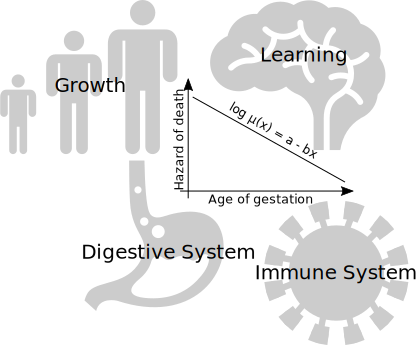
\includegraphics[width = \textwidth]{./fig/acquired_robustness.pdf}\\
\end{figure}

\column{0.25\textwidth}
\footnotesize\textbf{Acquired robustness}\\
Reduction of an individuals risk of death due to growth and adjustment.\\
\scriptsize\emph{cp.~\textcite{Levitis2011}, \textcite{Siler1979}}

\end{columns}

\end{frame}

\section{Ontogenescence as Transitional Timing} %%%%%%%%%%%%%%%%%%%%%%%%%%%%%%%

\begin{frame}
\frametitle{\insertsection}

\begin{columns}[c]

\column{0.5\textwidth}
\begin{figure}[htb!]
\caption{\textbf{Idealized individual hazard}\\over gestational age.}
\includegraphics[width = \textwidth]{./fig/birth_trauma.pdf}\\
\end{figure}

\column{0.5\textwidth}
\begin{figure}[htb!]
\caption{\textbf{US infant mortality 2009}\\by day of age.}
\includegraphics[width = \textwidth]{./fig/us_imort_2009_cumdx.pdf}\\
\end{figure}

\end{columns}

\vfill

\footnotesize\textbf{Transitional timing}~Early life is full of risky transitions which increase an individuals mortality risk. The process of birth is a prominent example. \scriptsize\emph{cp.~\textcite{Levitis2011}}

\end{frame}

\section{Ontogenescence as a Selection Process} %%%%%%%%%%%%%%%%%%%%%%%%%%%%%%%

\begin{frame}
\frametitle{\insertsection}

\begin{columns}[c]

\column{0.65\textwidth}
\begin{figure}[htb!]
\includegraphics[width = \textwidth]{./fig/plot-binary.pdf}\\
\end{figure}

\column{0.35\textwidth}
\footnotesize\textbf{The selection effect of heterogeneous frailties}\\
$h_{1,2}(x)$: Baseline hazard for two groups of different frailties\\
$\bar{h}(x)$: Mean hazard in the population\\
$p_1(x)$: Share of group 1 on the total population. \\ \scriptsize\emph{See \cite{Vaupel1985} for more of \enquote{Heterogeneity's Ruses}.}

\end{columns}

\end{frame}

\section{The Gestational Age Pattern of Human Mortality} %%%%%%%%%%%%%%%%%%%%%%

\begin{frame}
\frametitle{\insertsection}

\begin{figure}[htb!]
\includegraphics[width = 0.8\textwidth]{./fig/us_fimort_2009_mx.pdf}\\
\end{figure}

\footnotesize\textbf{Mortality rates by week of gestation}\\
A joint fetal-infant life table for the US conception cohort of 2009.\\
\scriptsize\emph{Raw~Data:~\textcite{DVS2015}; the mortality rates have been calculated by the author after aggregating individual records of births, fetal- and infant deaths.}

\end{frame}

%%%%%%%%%%%%%%%%%%%%%%%%%%%%%%%%%%%%%%%%%%%%%%%%%%%%%%%%%%%%%%%%%%%%%%%%%%%%%%%

\begin{frame}
\frametitle{\insertsection}

\begin{figure}[htb!]
\includegraphics[width = 0.8\textwidth]{./fig/us_fimort_2009_log_mx.pdf}\\
\end{figure}

\footnotesize\textbf{Mortality rates by week of gestation}\\
A joint fetal-infant life table for the US conception cohort of 2009.\\
\scriptsize\emph{Raw~Data:~\textcite{DVS2015}; the mortality rates have been calculated by the author after aggregating individual records of births, fetal- and infant deaths.}

\end{frame}

\section{Modelling the Pattern} %%%%%%%%%%%%%%%%%%%%%%%%%%%%%%%%%%%%%%%%%%%%%%%

\begin{frame}
\frametitle{\insertsection}

\begin{figure}[htb!]
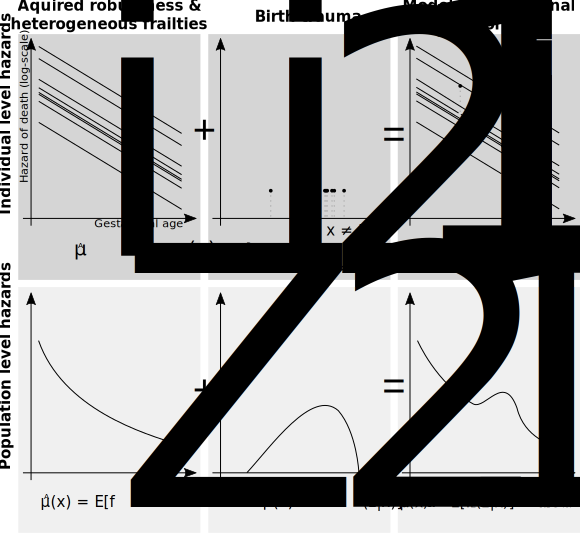
\includegraphics[width = 0.8\textwidth]{./fig/the_model.pdf}\\
\end{figure}

\end{frame}

%%%%%%%%%%%%%%%%%%%%%%%%%%%%%%%%%%%%%%%%%%%%%%%%%%%%%%%%%%%%%%%%%%%%%%%%%%%%%%%

\begin{frame}
\frametitle{\insertsection}

Modelling human ontogenescence across gestational age taking into account \emph{acquired robustness}, \emph{birth trauma} and \emph{selection}.

\begin{equation*}
  \underbrace{
    \overline{\mu}(x)
  }_{\substack{
    \text{Population hazard}\\ \text{at gestational age}~x
  }} =
  \underbrace{
    E[f_Z(z|x)]
  }_{\substack{
    \text{Average frailty}\\ \text{in population}\\ \text{at gestational age}~x
  }} \times
  \underbrace{
    \alpha_1 e^{-\lambda x}
  }_{\substack{
    \text{Acquired robustness}\\ \text{component of hazard}\\ \text{at gestational age}~x
  }} +
  \underbrace{
    \alpha_2 f_T(t).
  }_{\substack{
    \text{Birth trauma component}\\ \text{of hazard}\\ \text{at gestational age}~x.
  }}
\end{equation*}

\end{frame}

%%%%%%%%%%%%%%%%%%%%%%%%%%%%%%%%%%%%%%%%%%%%%%%%%%%%%%%%%%%%%%%%%%%%%%%%%%%%%%%

\begin{frame}
\frametitle{\insertsection}

Frailty is assumed to be \emph{Gamma} Distributed, the gestational age at onset of labour \emph{Beta} distributed.

\begin{equation*}
  \underbrace{
    \overline{\mu}(x)
  }_{\substack{
    \text{Population hazard}\\ \text{at gestational age}~x
  }} =
  \underbrace{
    \frac {\alpha_1 e^{-\lambda x}} {\frac{\gamma \alpha_1} {-\lambda} (e^{-\lambda x} - 1) + 1}
  }_{\substack{
    \text{Gamma-Gompertz}\\ \text{Frailty Model}
  }} +
  \underbrace{
    \frac{\alpha_2 x^{s_1-1} (24-x)^{s_2-1}} {B(s_1,s_2) \cdot 24^{s_1+s_2-1}}
  }_{\substack{
    \text{Birth trauma component}\\ \text{of hazard}\\ \text{at gestational age}~x.
  }}
\end{equation*}

\small\centering
\begin{tabular}{p{1cm}p{7cm}}
  $\alpha_1$ & The initial mortality level (at week 23 and process time 0). \\
  $\lambda$ & The relative rate of mortality decline over age. \\
  $\gamma$ & The initial variance of frailties in the population (at week 23 and process time 0).\\
  $\alpha_2$ & The added mortality risk due to the stress of birth. \\
  $s_1$ & The modal gestational age at onset of labour (in weeks after week 23). \\
  $s_2$ & The shape of the age distribution at onset of labour. \\
\end{tabular}

\end{frame}

%%%%%%%%%%%%%%%%%%%%%%%%%%%%%%%%%%%%%%%%%%%%%%%%%%%%%%%%%%%%%%%%%%%%%%%%%%%%%%%

\begin{frame}
\frametitle{\insertsection}

\begin{figure}[htb!]
\includegraphics[width = 0.8\textwidth]{./fig/us_fimort_2009_mx_predobs.pdf}\\
\end{figure}

\footnotesize\textbf{Mortality rates by week of gestation, observed versus predicted}\\
A joint fetal-infant life table for the US conception cohort of 2009.\\
\scriptsize\emph{Raw~Data:~\textcite{DVS2015}; the mortality rates have been calculated by the author after aggregating individual records of births, fetal- and infant deaths.}

\end{frame}

\section{Mortality Improvements by Gestational Age} %%%%%%%%%%%%%%%%%%%%%%%%%%%

\begin{frame}
\frametitle{\insertsection}

\begin{figure}[htb!]
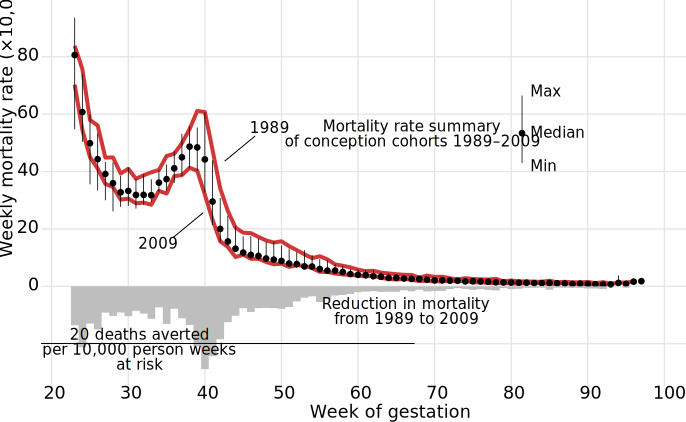
\includegraphics[width = 0.8\textwidth]{./fig/us_fimort_obsmx_1989_2009.pdf}\\
\end{figure}

\footnotesize\textbf{Mortality rates by week of gestation, different conception cohorts}\\
Based on single year conception cohorts 1989--2009. No data is available for the years 1991--1994.
\scriptsize\emph{Raw~Data:~\textcite{DVS2015}; the mortality rates have been calculated by the author after aggregating individual records of births, fetal- and infant deaths.}

\end{frame}

\section{References} %%%%%%%%%%%%%%%%%%%%%%%%%%%%%%%%%%%%%%%%%%%%%%%%%%%%%%%%%%

\begin{frame}
\frametitle{\insertsection}

\nocite{Hmd2015}

\printbibliography

\end{frame}

\end{document}